% DataAcquisitionSystem.tex
\section{Data Acquisition System}

% % for code listings
% \begin{lstlisting}[style=cstyle, caption=System Architecture Code Example, label=lst:SystemArchitecture8]
% # Your code here
% \end{lstlisting}

% % for figures
% \begin{figure}[htbp] %h-ere t-op b-ottom p-page (separte) -good to allow all htbp to give the compiler more options
%     \centering
%     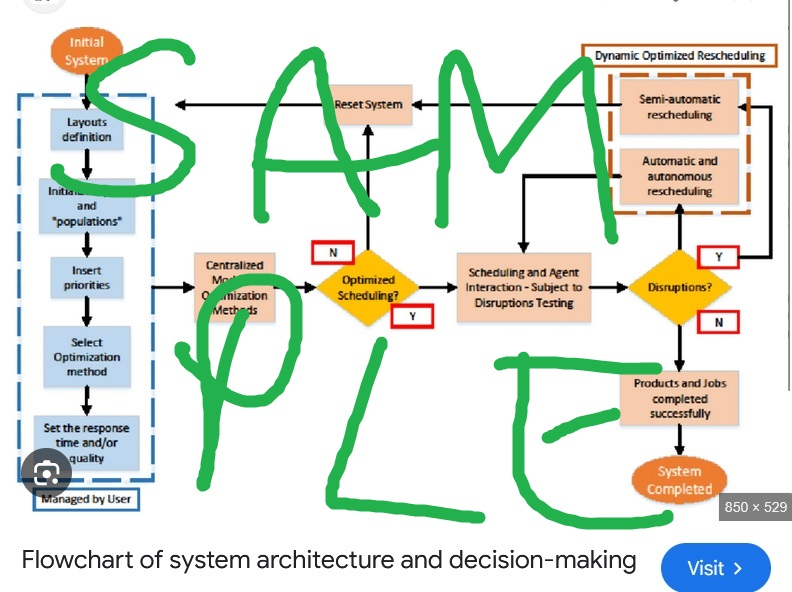
\includegraphics[width=0.6\textwidth]{figures/methodology/system_architecture.jpg}
%     \caption{System Architecture Diagram}
%     \label{fig:system-architecture3}
% \end{figure}

% % Include a flowchart in TEX mode
% \begin{figure}[H]
%     \centering
%     \scalebox{0.8}{ % Scale to 80% of original size
%         % try generating flowcharts as svg in Claude 
% and edit with inkscape instead of this.
% but claude did generate this one so might 
% be useful too but you can't easily make
% small repairs in inkscape


% CNN Transfer Learning Flowchart - Compact Multi-Column Layout
% \begin{figure}[htbp]

\centering
\resizebox{\textwidth}{!}{ % Scale to fit width while maintaining aspect ratio
\begin{tikzpicture}[node distance=0.8cm and 1.5cm, auto]
    % Define a smaller block style
    \tikzset{
      block/.style = {rectangle, draw, fill=blue!20, 
                      text width=7em, text centered, rounded corners, minimum height=1.8em, font=\small},
    }
    
    % Brazilian model training - Column 1
    \node [block] (brazildata) {Download Brazilian coins dataset};
    \node [block, below=of brazildata] (extract) {Extract dataset};
    \node [block, below=of extract] (setup) {Setup directories};
    \node [block, below=of setup] (define) {Define train/val dirs};
    \node [block, below=of define] (create) {Create CNN architecture};
    \node [block, below=of create] (compile) {Compile the CNN};
    \node [block, below=of compile] (train) {Train model};
    \node [block, below=of train] (trained) {Model trained (5 classes)};
    
    % Transfer learning - Column 2 (Middle)
    \node [block, right=2.5cm of brazildata] (freeze) {Freeze all layers};
    \node [block, below=of freeze] (replace) {Replace final layers};
    \node [block, below=of replace] (add) {Add regularization and dropout};
    \node [block, below=of add] (output) {New output layer (8 classes)};
    \node [block, below=of output] (finaltrain) {Train and fine-tune};
    \node [block, below=of finaltrain] (inference) {Perform inference on new coins};
    
    % UK data preparation - Column 3 (Right)
    \node [block, right=2.5cm of freeze] (ukdata) {Download UK coins dataset};
    \node [block, below=of ukdata] (ukextract) {Extract UK dataset};
    \node [block, below=of ukextract] (uksetup) {Setup UK directories};
    \node [block, below=of uksetup] (ukgen) {Create data generators (80/20 split)};
    
    % Connect all nodes with arrows
    \path [line] (brazildata) -- (extract);
    \path [line] (extract) -- (setup);
    \path [line] (setup) -- (define);
    \path [line] (define) -- (create);
    \path [line] (create) -- (compile);
    \path [line] (compile) -- (train);
    \path [line] (train) -- (trained);
    
    \path [line] (ukdata) -- (ukextract);
    \path [line] (ukextract) -- (uksetup);
    \path [line] (uksetup) -- (ukgen);
    
    % Connect the columns
    \path [line] (trained) -- node[midway, above] {Transfer} (freeze);
    \path [line] (ukgen) |- (finaltrain);
    
    % Connect middle column
    \path [line] (freeze) -- (replace);
    \path [line] (replace) -- (add);
    \path [line] (add) -- (output);
    \path [line] (output) -- (finaltrain);
    \path [line] (finaltrain) -- (inference);
    
    % Group boxes to show different stages with smaller padding
    \begin{pgfonlayer}{background}
        \node[group={[yshift=0.3cm]above:Brazilian Model Training}, fit={(brazildata) (extract) (setup) (define) (create) (compile) (train) (trained)}, inner sep=0.2cm] {};
        \node[group={[yshift=0.3cm]above:UK Data Preparation}, fit={(ukdata) (ukextract) (uksetup) (ukgen)}, inner sep=0.2cm] {};
        \node[group={[yshift=0.3cm]above:Transfer Learning}, fit={(freeze) (replace) (add) (output) (finaltrain) (inference)}, inner sep=0.2cm] {};
    \end{pgfonlayer}
\end{tikzpicture}
}
% \caption{CNN Transfer Learning Flowchart: Brazilian to UK Coins}
% \label{fig:cnn-flowchart}
% \end{figure} % \input is for tex files \includegraphics is for images
%     }
%     \caption{System Design Overview Flowchart}
%     \label{fig:decriptiveLabel22} % descriptive to call in text with \ref{fig:decriptiveLabel22}
% \end{figure}


% other subsections
\subsection{Functional Requirements}
% Your content here
The output signal from the photodiode array amplifier is required to be converted to digital form for post-processing. This requirement is filled by designing a Digital Acquisition System (DAQ) capable of recording the signal from the four photodiode circuits simultaneously.
The choice of design was conceived by analyzing the analog signal and determining some basic requirements of the Analog to Digital Converter (ADC) the DAQ must possess. 
%
% ANALOG SIGNAL CHARACTERISTICS
%
\paragraph{Analog Signal Characteristics}
\begin{itemize}
    \item The signal is four channel, one per photodiode, and between 0 and 5 Volts, as the TIA and post amplification was designed specifically for this output.
    \item Close to DC frequency, i.e., static in nature, due to light intensity remaining static under most tests. One test is performed at 0.2Hz, which is still still very low frequency, with the light completing a semicircular arc once in 130 seconds (26 positions of 5 seconds each). 
    \item Later in testing it was found that the signal is impacted by interference of 400mVpp at a frequency fluctuating from 160kHz to 180kHz from the RED testbench power supply, as pictured in Figure~\ref{fig:sigNoise}.
\end{itemize}
% for figures
\begin{figure}[htbp] 
    \centering
    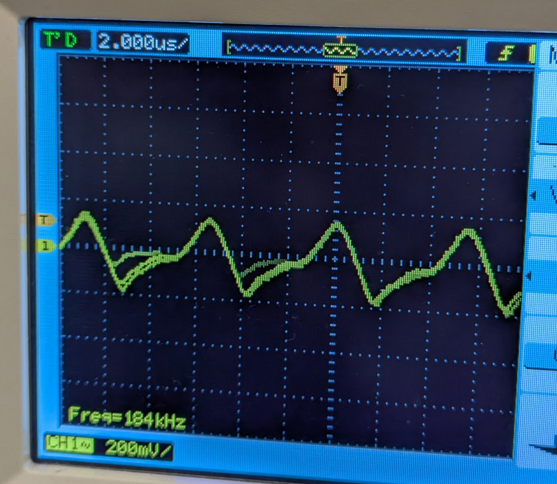
\includegraphics[width=0.4\textwidth]{chapters/methodology/ArduinoDAQ/signal_noise.png}
    \caption{Signal Noise Analysis, oscilloscope AC coupled}
    \label{fig:sigNoise}
\end{figure}
%
%     CSV DATA STRUCTURE
%
\paragraph{CSV Data Structure and Format Specification}is as follows:

The output of the DAQ is to be saved in Comma Separated Values (CSV) file format, with columns as follows: Sample(nr.), Time(ms), A0(V), A1(V), A2(V), A3(V). This allows for easy post-processing and plotting.
\subsection{Design Approach}
The characteristics of the signal being low frequency, combined with the requirement to read all four signals simultanously and in sync, meant two things: the Sampling Rate could be quite low due to Nyquist theorem telling us that the sampling rate must be at least twice the frequency of the signal being sampled, in order to maintain the original signal without aliasing~\cite[p. 146]{RefWorks:schafer2013discrete-time}. Therefore a low performing ADC is acceptable for a signal changing at under 1Hz. And secondly, the DAQ must support sampling from at least four analog inputs. These requirements meant that a cheap Arduino based DAQ could fit perfectly the needs of the project: it is powered by the Atmega328P which has an included ADC of 15 ksps~\cite[p.205]{RefWorks:atmel2015atmega328p}. And the Arduino Nano has four analog inputs. 
\subsubsection{Arduino Programming}
The Arduino-based DAQ will require both a C++ program written for the Arduino itself, as well as a program or script on the PC receiving the digitized signal, this is because the Arduino lacks both the memory requirements and capability to store the recorded digitized signal to some internal memory.
\paragraph{The Arduino C++ Program} must be able to listen to commands from the user on the PC receiving, start a recording, and immediatly transmit to the PC over serial communication. 

\subsection{Technical Specifications}


\subsubsection{Arduino Code}
The Arduino Code which uses the Arduino ADC is formed of the setup() function triggered once at the start/reset of the device and a standard contnuous loop triggered after setup comletes. Inside the loop, two if statements check for instructions from the PC script. The recording time limit is hardcoded as a global function. Figure~\ref{fig:arduinoPseudoCodeFlowchart} shows the algorithm that checks for Serial data in, waits for a command to start recording, and if recording time has reached the preset limit, it stops recoring, sends the last values to the Python script on the PC and a "recording\_stopped" command. The pseudocode used while designing the Arduino side of the DAQ system, is available in Listing~\ref{lst:arduinoPseudoCode}. The final code is available in Appendix \ref{subsec:arduinoCppcode}.
\paragraph{The Atmega328P} does not have a separate ADC clock input, therefore the CPU clock is used by first dividing by a default rate of 128, this divider is changed to 16 by changing bits 2-0 to 100, as per~\cite[p.219]{RefWorks:atmel2015atmega328p}. This increases the clock speed available to the ADC for a higher sampling rate. This results in a 1MHz clock signal to the ADC (16MHz/16) which seemed needed when dealing with multiplexing four analog inputs to a single ADC. The process is as follows:


Original ADC Clock Speed (with default prescaler of 128):
\begin{equation} \label{origclk}
  \begin{split}
f_\text{ADC-default} = \frac{f_\text{CPU}}{Prescaler_\text{default}} = \frac{16 \text{ MHz}}{128} = 125 \text{ kHz}
  \end{split}
\end{equation}
\addequation{Default ADC Clock Frequency Calculation}

Optimized ADC Clock Speed (with modified prescaler of 16):
\begin{equation} \label{optimizedclk}
  \begin{split}
f_\text{ADC-optimized} = \frac{f_\text{CPU}}{Prescaler_\text{optimized}} = \frac{16 \text{ MHz}}{16} = 1 \text{ MHz}
\end{split}
\end{equation}
\addequation{Optimized ADC Clock Frequency Calculation}

Conversion Time Calculations:
ADC requires approximately 13 clock cycles for each conversion~\cite[p.208]{RefWorks:atmel2015atmega328p}
Optimized ADC Clock Speed (with modified prescaler of 16):
\begin{equation} \label{optimCLKspeed}
  \begin{split}
T_\text{conversion-default} = 13 \times \frac{1}{f_\text{ADC-default}} = 13 \times \frac{1}{125 \text{ kHz}} \approx 104 \text{ $\mu$s}
  \end{split}
\end{equation}
\addequation{Default ADC Conversion Time}

\begin{equation} \label{optimCLKspeed2}
  \begin{split}
T_\text{conversion-optimized} = 13 \times \frac{1}{f_\text{ADC-optimized}} = 13 \times \frac{1}{1 \text{ MHz}} \approx 13 \text{ $\mu$s}
  \end{split}
\end{equation}
\addequation{Optimized ADC Conversion Time}

Time required to sample all 4 analog inputs:
\begin{equation} \label{T4analogIn}
  \begin{split}
T_\text{4channels-default} = 4 \times T_\text{conversion-default} = 4 \times 104 \text{ $\mu$s} \approx 416 \text{ $\mu$s}
\end{split}
\end{equation}
\addequation{Total Sampling Time for 4 Channels (Default)}

\begin{equation} \label{T4analogIn2}
  \begin{split}
T_\text{4channels-optimized} = 4 \times T_\text{conversion-optimized} = 4 \times 13 \text{ $\mu$s} \approx 52 \text{ $\mu$s}
\end{split}
\end{equation}
\addequation{Total Sampling Time for 4 Channels (Optimized)}

Maximum theoretical sampling frequency for all 4 channels:
\begin{equation} \label{Tmax4ch}
  \begin{split}
f_\text{sampling-max-default} = \frac{1}{T_\text{4channels-default}} = \frac{1}{416 \text{ $\mu$s}} \approx 2.4 \text{ kHz}
\end{split}
\end{equation}
\addequation{Maximum Theoretical Sampling Frequency (Default)}

\begin{equation} \label{Tmax4ch2}
  \begin{split}
f_\text{sampling-max-optimized} = \frac{1}{T_\text{4channels-optimized}} = \frac{1}{52 \text{ $\mu$s}} \approx 19.2 \text{ kHz}
\end{split}
\end{equation}
\addequation{Maximum Theoretical Sampling Frequency (Optimized)}

Actual limited sampling frequency (based on minSampleInterval = 2ms):
\begin{equation} \label{Tlim2ms}
  \begin{split}
f_\text{sampling-actual} = \frac{1}{2 \text{ ms}} = 500 \text{ Hz} \text{ per channel}
\end{split}
\end{equation}
\addequation{Actual Limited Sampling Frequency}

Effective data rate across all channels:
\begin{equation} \label{EffectiveDATArate}
  \begin{split}
\text{Data Rate} = 4 \text{ channels} \times 500 \text{ Hz} = 2000 \text{ samples/second}
\end{split}
\end{equation}
\addequation{Total Effective Data Rate}

\subsubsection{Python Script}
The digitized signal must be interpreted and saved on the PC. This is done via a python script
% Flowchart Arduino Code
\begin{figure}[p] %h-ere t-op b-ottom p-page (separte) -good to allow all htbp to give the compiler more options
    \centering
    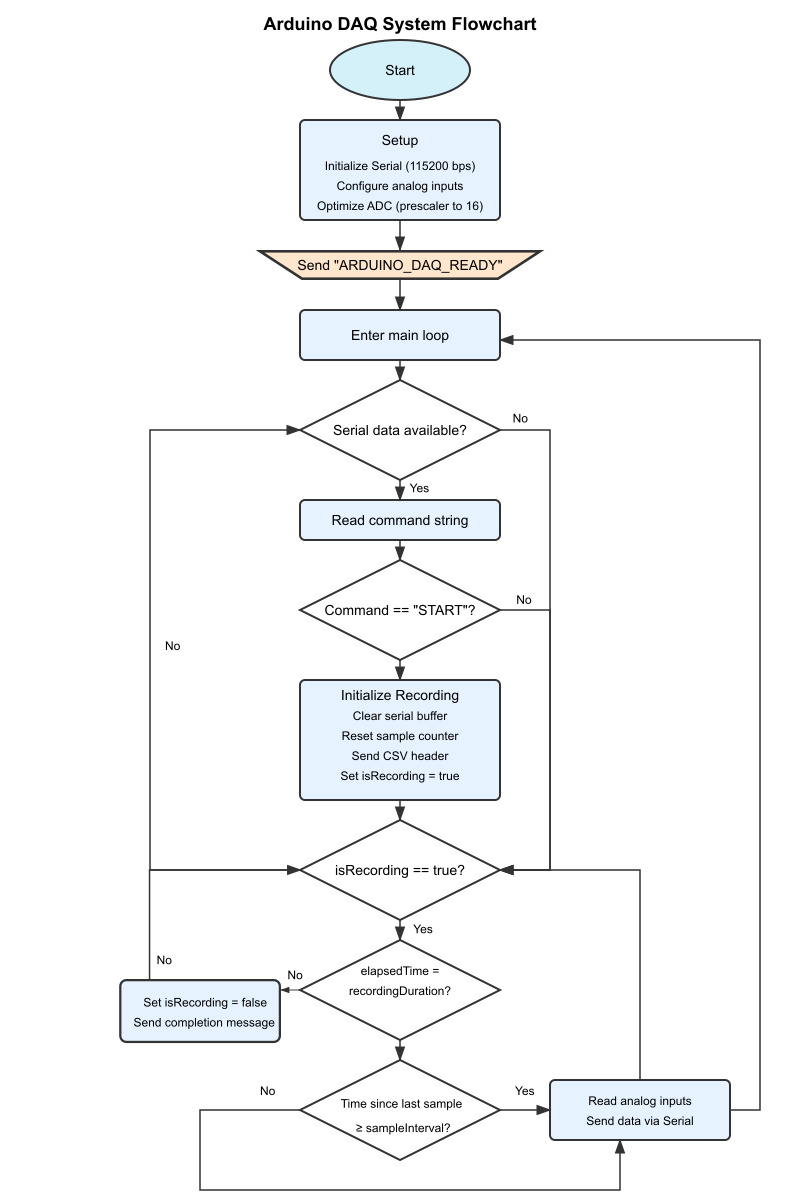
\includegraphics[width=0.95\textwidth]{chapters/methodology/ArduinoDAQ/flowchart_Arduino_code.png}
    \caption{Flowchart Arduino DAQ C++ program}
    \label{fig:arduinoPseudoCodeFlowchart}
\end{figure}

%%% Arduino CPP pseudocode
\begin{lstlisting}[style=cstyle, caption=Arduino DAQ PseudoCode, label=lst:arduinoPseudoCode]
  recordingDuration = 5000 // for how long to record in milliseconds
  
  minSampleInterval = 2    // control how fast to sample to avoid
                           // relying on Arduino performance
  // Initialize serial communication
  // Initialize analog inputs
  // Setup ADC

  // Infrom PC listening on Serial Connection: Arduino is ready to record
  Serial.print("Arduino_DAQ_Ready")
  // enter the loop 
  void loop(){
    //listen for command from PC script:
      String command = Serial.read()
    //set system state
    if (command == "START"){
      // Send header of csv
      Serial.println("Sample,Time(ms),A0(V),A1(V),A2(V),A3(V)")
      // keep track of system state
      state = recording
      // keep time
      startTime = currentTime()
      // send confirmation
      Serial.println("recording in progress")
      }
    // check if recording
    if (state == recording){
      // check if within recording period
      currentTime = currentTime()
      elapsedTime = currentTime - startTime
      if(currentTime <= recordingDuration){
        // Also check not recording too fast  
        if(currentTime - lastSampleTime >= minSampleInterval){
          sampleCount++;
          // Start each row with sample count and time of sample
          String currentCSVrow = String(sampleCount) , string(elapsedTime)
          // Multiplex through all analog inputs 
          for (int = 0;i<4;i++){
            //read raw values
            rawValue = analogRead(analogInputs[i]);
            // compute real value
            voltage = rawValue * 5/1023
            // add value to current row to send
            currentCSVrow += String(voltage)
            }
          // Send completed row to PC
          Serial.println(currentCSVrow)
          }
        }
      }
  // end recording
  else{
    state = notRecording
    // tell PC recording finished
    Serial.println("Recording_finished")
    }
  }
  \end{lstlisting}
                          
\paragraph{Sampling Rate}
Several factors restrict the sampling rate:

\subparagraph{Sample Interval Setting}
The most direct limitation is the \texttt{sampleInterval} constant set to 2ms in the code, which means samples are taken no more frequently than every 2 milliseconds (500 Hz theoretical maximum).

\subparagraph{ADC Prescaler Configuration}
The ADC prescaler is set to 16 (from the default of 128) with this line:
\begin{verbatim}
ADCSRA = (ADCSRA & 0xF8) | 0x04;
\end{verbatim}
This increases the ADC clock to 16MHz/16 = 1MHz. With each conversion taking 13 ADC clock cycles, the theoretical maximum sampling rate is about 76.9kHz for a single channel.

\subparagraph{Multiple Channel Reading}
Since the system reads from 4 analog inputs sequentially, the effective per-channel sampling rate is reduced by approximately a factor of 4.

\subparagraph{Serial Transmission Overhead}
Each sample requires formatting and sending data over serial:
\begin{verbatim}
String dataString = String(sampleCount) + "," + String(elapsedTime);
// ... format and add voltage values ...
Serial.println(dataString);
\end{verbatim}
This string creation and serial transmission takes considerable time.

\subparagraph{Serial Baud Rate}
The code uses 115200 bps, which limits how quickly data can be transmitted. Each sample in this format might be around 30-40 bytes, which means \texttildelow 3000-3800 samples/second theoretical maximum throughput.

\subparagraph{String Operations}
The use of the Arduino \texttt{String} class is memory-intensive and can cause fragmentation over time, potentially causing slowdowns.

\subparagraph{Loop Cycle Time}
Other operations in the main loop consume processing time.

The dominant limiting factor in this implementation is likely the combination of the explicit 2ms sample interval and the serial communication overhead. Higher sampling rates would require optimizing the data transmission format, possibly using binary rather than text formatting, and reducing the sample interval.
